\documentclass[twoside]{book}

% Packages required by doxygen
\usepackage{fixltx2e}
\usepackage{calc}
\usepackage{doxygen}
\usepackage[export]{adjustbox} % also loads graphicx
\usepackage{graphicx}
\usepackage[utf8]{inputenc}
\usepackage{makeidx}
\usepackage{multicol}
\usepackage{multirow}
\PassOptionsToPackage{warn}{textcomp}
\usepackage{textcomp}
\usepackage[nointegrals]{wasysym}
\usepackage[table]{xcolor}

% Font selection
\usepackage[T1]{fontenc}
\usepackage[scaled=.90]{helvet}
\usepackage{courier}
\usepackage{amssymb}
\usepackage{sectsty}
\renewcommand{\familydefault}{\sfdefault}
\allsectionsfont{%
  \fontseries{bc}\selectfont%
  \color{darkgray}%
}
\renewcommand{\DoxyLabelFont}{%
  \fontseries{bc}\selectfont%
  \color{darkgray}%
}
\newcommand{\+}{\discretionary{\mbox{\scriptsize$\hookleftarrow$}}{}{}}

% Page & text layout
\usepackage{geometry}
\geometry{%
  a4paper,%
  top=2.5cm,%
  bottom=2.5cm,%
  left=2.5cm,%
  right=2.5cm%
}
\tolerance=750
\hfuzz=15pt
\hbadness=750
\setlength{\emergencystretch}{15pt}
\setlength{\parindent}{0cm}
\setlength{\parskip}{3ex plus 2ex minus 2ex}
\makeatletter
\renewcommand{\paragraph}{%
  \@startsection{paragraph}{4}{0ex}{-1.0ex}{1.0ex}{%
    \normalfont\normalsize\bfseries\SS@parafont%
  }%
}
\renewcommand{\subparagraph}{%
  \@startsection{subparagraph}{5}{0ex}{-1.0ex}{1.0ex}{%
    \normalfont\normalsize\bfseries\SS@subparafont%
  }%
}
\makeatother

% Headers & footers
\usepackage{fancyhdr}
\pagestyle{fancyplain}
\fancyhead[LE]{\fancyplain{}{\bfseries\thepage}}
\fancyhead[CE]{\fancyplain{}{}}
\fancyhead[RE]{\fancyplain{}{\bfseries\leftmark}}
\fancyhead[LO]{\fancyplain{}{\bfseries\rightmark}}
\fancyhead[CO]{\fancyplain{}{}}
\fancyhead[RO]{\fancyplain{}{\bfseries\thepage}}
\fancyfoot[LE]{\fancyplain{}{}}
\fancyfoot[CE]{\fancyplain{}{}}
\fancyfoot[RE]{\fancyplain{}{\bfseries\scriptsize Generated by Doxygen }}
\fancyfoot[LO]{\fancyplain{}{\bfseries\scriptsize Generated by Doxygen }}
\fancyfoot[CO]{\fancyplain{}{}}
\fancyfoot[RO]{\fancyplain{}{}}
\renewcommand{\footrulewidth}{0.4pt}
\renewcommand{\chaptermark}[1]{%
  \markboth{#1}{}%
}
\renewcommand{\sectionmark}[1]{%
  \markright{\thesection\ #1}%
}

% Indices & bibliography
\usepackage{natbib}
\usepackage[titles]{tocloft}
\setcounter{tocdepth}{3}
\setcounter{secnumdepth}{5}
\makeindex

% Hyperlinks (required, but should be loaded last)
\usepackage{ifpdf}
\ifpdf
  \usepackage[pdftex,pagebackref=true]{hyperref}
\else
  \usepackage[ps2pdf,pagebackref=true]{hyperref}
\fi
\hypersetup{%
  colorlinks=true,%
  linkcolor=blue,%
  citecolor=blue,%
  unicode%
}

% Custom commands
\newcommand{\clearemptydoublepage}{%
  \newpage{\pagestyle{empty}\cleardoublepage}%
}

\usepackage{caption}
\captionsetup{labelsep=space,justification=centering,font={bf},singlelinecheck=off,skip=4pt,position=top}

%===== C O N T E N T S =====

\begin{document}

% Titlepage & ToC
\hypersetup{pageanchor=false,
             bookmarksnumbered=true,
             pdfencoding=unicode
            }
\pagenumbering{roman}
\begin{titlepage}
\vspace*{7cm}
\begin{center}%
{\Large \textquotesingle{}Exam\+\_\+\+C\+PP\textquotesingle{} }\\
\vspace*{1cm}
{\large Generated by Doxygen 1.8.11}\\
\end{center}
\end{titlepage}
\clearemptydoublepage
\tableofcontents
\clearemptydoublepage
\pagenumbering{arabic}
\hypersetup{pageanchor=true}

%--- Begin generated contents ---
\chapter{Class Index}
\section{Class List}
Here are the classes, structs, unions and interfaces with brief descriptions\+:\begin{DoxyCompactList}
\item\contentsline{section}{\hyperlink{classmenu}{menu} \\*Classe menu contenant plusieurs methodes pour afficher et éxécuter les options du menu }{\pageref{classmenu}}{}
\end{DoxyCompactList}

\chapter{File Index}
\section{File List}
Here is a list of all documented files with brief descriptions\+:\begin{DoxyCompactList}
\item\contentsline{section}{/home/euphoria/\+Documents/cours\+\_\+b2/c\+\_\+c++/b2/exam\+\_\+cpp/src/\hyperlink{menu_8h}{menu.\+h} \\*Fichier de la classe menu }{\pageref{menu_8h}}{}
\end{DoxyCompactList}

\chapter{Class Documentation}
\hypertarget{classmenu}{}\section{menu Class Reference}
\label{classmenu}\index{menu@{menu}}


classe menu contenant plusieurs methodes pour afficher et éxécuter les options du menu.  




{\ttfamily \#include $<$menu.\+h$>$}

\subsection*{Public Member Functions}
\begin{DoxyCompactItemize}
\item 
int \hyperlink{classmenu_aae6b44c64a4e429c54640a5a246e94b3}{select} ()\hypertarget{classmenu_aae6b44c64a4e429c54640a5a246e94b3}{}\label{classmenu_aae6b44c64a4e429c54640a5a246e94b3}

\begin{DoxyCompactList}\small\item\em methode selection, affiche le menu \end{DoxyCompactList}\item 
void \hyperlink{classmenu_a6fd4100786d389ca943629755eff3936}{add} ()\hypertarget{classmenu_a6fd4100786d389ca943629755eff3936}{}\label{classmenu_a6fd4100786d389ca943629755eff3936}

\begin{DoxyCompactList}\small\item\em methode add, ajoute un élément à la liste \end{DoxyCompactList}\item 
void \hyperlink{classmenu_aae1769c812999eba1699adcf91481a06}{show} ()\hypertarget{classmenu_aae1769c812999eba1699adcf91481a06}{}\label{classmenu_aae1769c812999eba1699adcf91481a06}

\begin{DoxyCompactList}\small\item\em methode show, montre la liste \end{DoxyCompactList}\item 
void \hyperlink{classmenu_a5f9e06b936a77a98f8202dd05524ca42}{delete\+\_\+first} ()\hypertarget{classmenu_a5f9e06b936a77a98f8202dd05524ca42}{}\label{classmenu_a5f9e06b936a77a98f8202dd05524ca42}

\begin{DoxyCompactList}\small\item\em methode delete\+\_\+first, supprime le premier élément donné \end{DoxyCompactList}\item 
void \hyperlink{classmenu_a051fef5d59afc3462896fa74cad3c598}{delete\+\_\+all} ()\hypertarget{classmenu_a051fef5d59afc3462896fa74cad3c598}{}\label{classmenu_a051fef5d59afc3462896fa74cad3c598}

\begin{DoxyCompactList}\small\item\em methode delete\+\_\+all, supprime tous les éléments donnés \end{DoxyCompactList}\item 
void \hyperlink{classmenu_aa1c97c7187ff0fd1744fcd2e42c3910c}{exit} ()\hypertarget{classmenu_aa1c97c7187ff0fd1744fcd2e42c3910c}{}\label{classmenu_aa1c97c7187ff0fd1744fcd2e42c3910c}

\begin{DoxyCompactList}\small\item\em methode delete\+\_\+all, enregistre la liste dans un fichier txt et quitte l\textquotesingle{}application \end{DoxyCompactList}\end{DoxyCompactItemize}
\subsection*{Public Attributes}
\begin{DoxyCompactItemize}
\item 
vector$<$ float $>$ {\bfseries tab}\hypertarget{classmenu_a9482736291bba796d0daecdc91ef21c8}{}\label{classmenu_a9482736291bba796d0daecdc91ef21c8}

\end{DoxyCompactItemize}
\subsection*{Static Public Attributes}
\begin{DoxyCompactItemize}
\item 
static int {\bfseries compteur} =0\hypertarget{classmenu_a8fc38c22ece04ea5f34301b225d66644}{}\label{classmenu_a8fc38c22ece04ea5f34301b225d66644}

\end{DoxyCompactItemize}


\subsection{Detailed Description}
classe menu contenant plusieurs methodes pour afficher et éxécuter les options du menu. 

The documentation for this class was generated from the following files\+:\begin{DoxyCompactItemize}
\item 
/home/euphoria/\+Documents/cours\+\_\+b2/c\+\_\+c++/b2/exam\+\_\+cpp/src/\hyperlink{menu_8h}{menu.\+h}\item 
/home/euphoria/\+Documents/cours\+\_\+b2/c\+\_\+c++/b2/exam\+\_\+cpp/src/menu.\+cpp\end{DoxyCompactItemize}

\chapter{File Documentation}
\hypertarget{menu_8h}{}\section{/home/euphoria/\+Documents/cours\+\_\+b2/c\+\_\+c++/b2/exam\+\_\+cpp/src/menu.h File Reference}
\label{menu_8h}\index{/home/euphoria/\+Documents/cours\+\_\+b2/c\+\_\+c++/b2/exam\+\_\+cpp/src/menu.\+h@{/home/euphoria/\+Documents/cours\+\_\+b2/c\+\_\+c++/b2/exam\+\_\+cpp/src/menu.\+h}}


fichier de la classe menu  


{\ttfamily \#include $<$string$>$}\\*
{\ttfamily \#include $<$iostream$>$}\\*
{\ttfamily \#include $<$vector$>$}\\*
{\ttfamily \#include $<$algorithm$>$}\\*
{\ttfamily \#include $<$fstream$>$}\\*
Include dependency graph for menu.\+h\+:\nopagebreak
\begin{figure}[H]
\begin{center}
\leavevmode
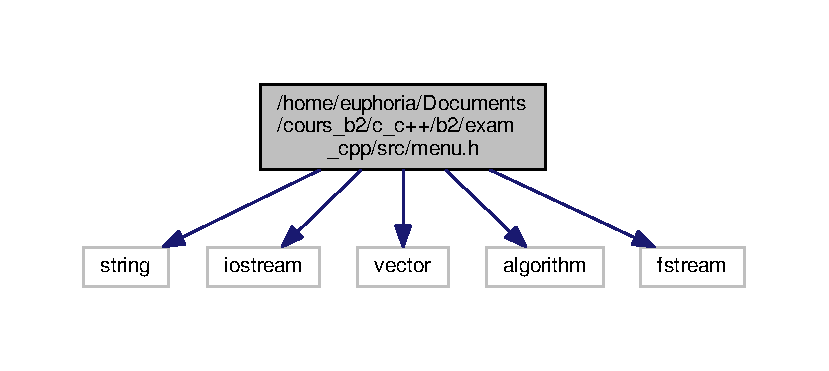
\includegraphics[width=350pt]{menu_8h__incl}
\end{center}
\end{figure}
\subsection*{Classes}
\begin{DoxyCompactItemize}
\item 
class \hyperlink{classmenu}{menu}
\begin{DoxyCompactList}\small\item\em classe menu contenant plusieurs methodes pour afficher et éxécuter les options du menu. \end{DoxyCompactList}\end{DoxyCompactItemize}


\subsection{Detailed Description}
fichier de la classe menu 

\begin{DoxyAuthor}{Author}
Paul 
\end{DoxyAuthor}
\begin{DoxyVersion}{Version}
1.\+0 
\end{DoxyVersion}

%--- End generated contents ---

% Index
\backmatter
\newpage
\phantomsection
\clearemptydoublepage
\addcontentsline{toc}{chapter}{Index}
\printindex

\end{document}
